\subsection{Child Persona}
\label{sub:child_persona}

\marginpar{%
	\null
	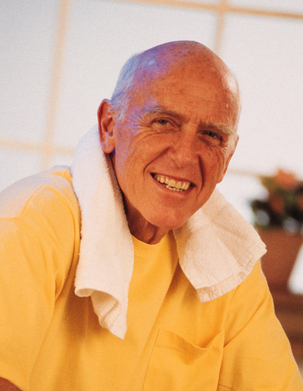
\includegraphics[width=\marginparwidth]{img/personas/elderly.jpg}
	\medskip
	\begin{description}[leftmargin=3cm]
		\item[Name] Joe Wyatt
		\item[Occupation] School student
		\item[Age] 14
	\end{description}

	\subsection*{Main Goals}
	\begin{itemize}[leftmargin=1em]
		\item Stay active and have fun playing sports, with his father if possible.
		\item Try out new sports
		\item Make friends
	\end{itemize}
}

\subsubsection*{Description}
\label{ssub:child_description}

Joe lives at home in a small town with his father, Pete. He is very active,
playing many sports at school and outside and enjoys trying new sports whenever
the opportunity is available. His father is keen to encourage him to
participate in a wide range of activities so that he can make friends and stay
fit.

Joe is at school every day, but has afternoons after school, and the weekends
available. His father tries to find times when they can spend time together so
sometimes take an afternoon off work to play sport with Joe.

Pete commutes just a short way to work by car, so doesn't mind travelling a bit
to find some good facilities and has also been very active in the past so is
always up for trying out new sports.

Joe is very adept with the latest technology, but occasionally has difficulty
with words and colours since he has very mild dyslexia and red-green
colorblindness.

% subsubsection description (end)

\subsubsection*{Scenarios}
\label{ssub:child_scenarios}

\begin{itemize}
	\item With summer approaching, Joe wants to start a new sport outside and
		his dad wants him to have a professional coach. He's not too concerned
		what it is, but it needs to be close to home, as he'll need to get the
		bus there.

	\item Its the end of term and Joe wants to organise a squash tournament
		with a group of friends and his Dad. They want to book a couple of
		courts nearby for after school during the week, but they're not to
		concerned about the day.

	\item Pete and Joe want to play a game of tennis, but the court they
		sometimes go to is not of great quality. This time, they don't mind
		going further, and want to spend a bit more to get really good courts.
\end{itemize}

% subsubsection scenarios (end)

\subsubsection*{Pain Points}
\label{ssub:child_pain_points}

\begin{itemize}
	\item Sometimes has difficulty reading small text with bad colours.
	\item Pete is keen to get a good deal whenever possible, but not at the
		expense of good facilities at the right time.
\end{itemize}

% subsubsection pain_points (end)
